\section{Navigation}\label{sec:navigation}
As mention in the previous Section we use of the navigation drawer in our application, the navigation drawer is a navigation design pattern acknowledged and used by Google.\cite{guidelines-navigationdrawer}
The navigation drawer is a powerful design on Android that allows the user from any views in the application to navigate to top level views. The navigation drawer is expanded from the 
left of the application.
\begin{figure}[H]
\centering
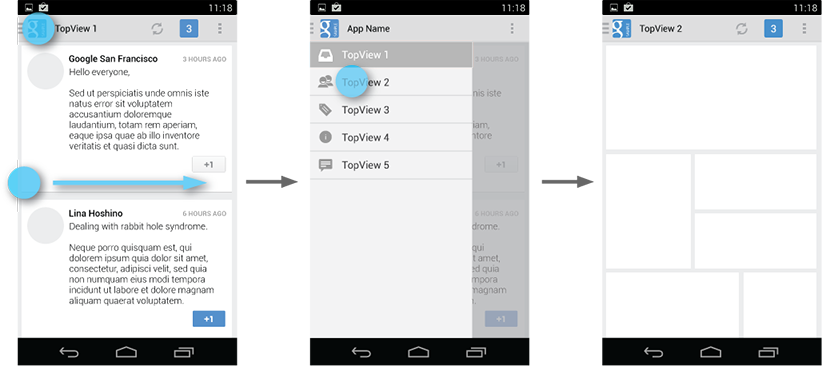
\includegraphics[width=0.9\linewidth]{img/screenshots/navigation_drawer_overview.png}
\caption{Navigation drawer overview}
\label{fig:navigationdrawer}
\end{figure}
\todo{insert picture of a expanded navigation drawer} There are two different ways of expanding the navigation drawer, the consistent one being swiping from the left edge of the screen to the centre. The second one being pressing the button in the top left, the button the marked with three lines, The \autoref{fig:navigationdrawer} illustrates this. Each item in the navigation drawer navigates to different top-level pages in the application, or typical main actions like sign in/sign out. 